\documentclass{article}

\usepackage[T1]{fontenc}
\usepackage[utf8]{inputenc}
\usepackage[brazilian]{babel}
\usepackage{graphicx}
\usepackage[export]{adjustbox}[2011/08/13]
\usepackage{float}
\usepackage[pdftex]{hyperref}
\usepackage{epstopdf}
\usepackage{etoolbox}
\usepackage{amsmath}
\usepackage{amsfonts}
\usepackage{amssymb}
\usepackage{caption}
\usepackage{subcaption}
\usepackage{setspace}
\usepackage{tikz}
\usepackage{listings}
\usepackage{xcolor} 

\bibliographystyle{eric}
\patchcmd{\thebibliography}{\section*}{\section}{}{}


\newcommand{\R}{\ensuremath{\mathbb{R}}}
\newcommand{\Prob}{\ensuremath{\mathbb{P}}}
\newcommand{\K}{\ensuremath{\mathbb{K}}}
\newcommand{\U}{\ensuremath{\mathbb{U}}}
\newcommand{\N}{\ensuremath{\mathbb{N}}}
\newcommand{\Lg}{\ensuremath{\mathbb{L}}}
\newcommand{\T}{\ensuremath{\rm Tr}}
\newcommand{\sg}{{\sigma(x_k)}}

\newcommand{\G}{\ensuremath{\mathcal{G}}}
\newcommand{\F}{\ensuremath{\mathcal{F}}}
\newcommand{\C}{\ensuremath{\mathcal{C}}}
\newcommand{\E}{\ensuremath{\mathcal{E}}}
\newcommand{\Hn}{\ensuremath{\mathcal{H}}}
\newcommand{\Hoo}{\ensuremath{\mathcal{H}_\infty}}
\newcommand{\Hop}{\ensuremath{\mathcal{H}_{op}}}
% --------------------------------------------------
\newtheorem{theo}{Teorema}
\newtheorem{exa}{Exemplo}
\newtheorem{lemm}{Lema}
\newtheorem{coro}{Corolário}
\newtheorem{defn}{Definição}[section]

\begin{document}

\begin{titlepage}
\begin{center}

\newcommand{\HRule}{\rule{\linewidth}{0.5mm}}
% Upper part of the page. The '~' is needed because \\
% only works if a paragraph has started.

\includegraphics[width=0.15\textwidth]{logoUnicamp}~\\[1cm]

\textsc{\LARGE Universidade Estadual de Campinas}\\[1.5cm]

\textsc{\Large Faculdade de Engenharia Mecânica}\\[0.5cm]

% Title
\HRule \\[0.4cm]
{ \huge \bfseries ES664 - Laboratório de Eletrônica para Automação Industrial\\ \vspace{1cm} Relatório - Experimento 4\\
\Large{Acionamento de motor DC} \\[0.4cm] }

\HRule \\[1.5cm]

% Author and supervisor
\begin{minipage}{0.6\textwidth}
\begin{flushleft} \large
\emph{Nome:}\\
Daniel Dello Russo Oliveira\\Marcelli Tiemi Kian
\end{flushleft}
\end{minipage}
\begin{minipage}{0.2\textwidth}
\begin{flushright} \large
\emph{RA}\\ 101918\\117892
\end{flushright}
\end{minipage}

\vfill

% Bottom of the page
{\large \today}

\end{center}
\end{titlepage}


\onehalfspacing
\section{Objetivos}
	O experimento tem como objetivo implementar o acionamento de um motor DC através de um retificador controlado e um chopper. Além disso, queremos avaliar o controle de velocidade do motor em malha aberta.
	 
\section{Experimento}
\subsection{Retificador Monofásico Controlado}
Utilizamos um transformador para rebaixar a tensão de $220\ V$ para $24\ V$, fazendo a ligação da tensão de linha (protegida pelos fusíveis) no primário, obtendo como saída $25.54\ V$. No secundário, ligamos o circuito na entrada do conversor. Alimentamos e configuramos o cartão de disparos, permitindo configurar $\alpha$ por meio de um potenciômetro. O esquemático do sistema pode ser visto na figura \ref{fig:retesq}.

\begin{figure}[H]
	\centering
	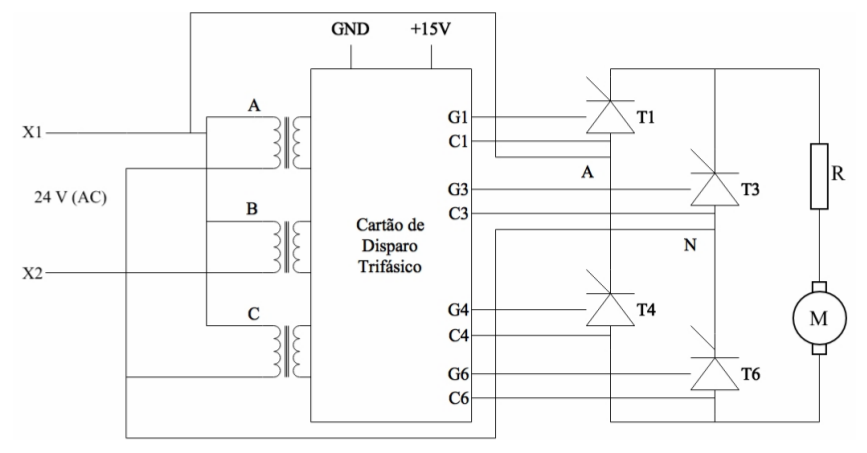
\includegraphics[width=\linewidth]{Dados/Retificador/esq}
	\caption{Retificador monofásico controlado de onda completa utilizado para acionar motor DC. (roteiro)}
	\label{fig:retesq}
\end{figure}

Prosseguimos o experimento com a medição da resistência de armadura do motor:
\begin{equation}
R_a=7.9\ \Omega
\end{equation}
e com a resistência de medição 
\begin{equation}
R_R=3.8\ \Omega
\end{equation}
sendo este último valor diferente do sugerido no roteiro ($0.2\Omega$).

Ligamos o circuito e capturamos a forma de onda da tensão de armadura $v_a$ para $\alpha=90^\circ$, conforme figura \ref{fig:varet}. Variando os valores de $\alpha$, obtivemos os valores da tabela \ref{tab:varet}. Por um erro de medição, essa tensão medida é na realidade a soma da tensão aplicada sobre a armadura do circuito e sobre o resistor de medição.

Medimos também a tensão no resistor de medição $R_R$, para cálculo da corrente de armadura, conforme figura \ref{fig:iaret} e equação abaixo. Conforme orientado pelo professor, descontinuamos o experimento sem fazer a medição da corrente para outros valores de $\alpha$. 
\begin{equation}
i_a=\frac{v_R}{R_R}
\end{equation}

Calculamos o torque no motor a fazendo a substituição nos valores da equação abaixo, em que igualamos a potência mecânica com a potência elétrica (descontando a potência dissipada na armadura), e isolamos a variável de torque.
\begin{equation}
T_m=\frac{v_a*i_a - R_a i_a^2}{\omega_m}
\label{eq:conserv}
\end{equation}
Sabemos que: 
\begin{equation}
T_m = k_t i_a
\end{equation}
\begin{equation}
V_e = k_e \omega_m
\end{equation}
\begin{equation}
V_a = R_a i_a + L_a\frac{di_a}{dt} + V_e
\end{equation}
Considerando que estamos trabalhando com valores médios e em regime permanente e que a tensão medida incluí a tensão sobre o resistor de medição, podemos escrever as equações acima como:
\begin{equation}
i_a = \frac{V_a - k_e\omega_m}{R_a + R_R}
\label{eq:retia}
\end{equation}
\begin{equation}
T_m = k_t i_a
\label{eq:rettm}
\end{equation}
Encontramos, para $\alpha = 90^\circ$, $k_t = 0,0536 N m/A$ e $k_e = 0,0536 V s/rad$. Sabemos que $k_t$ e $k_e$ deveriam apresentar o mesmo valor quando escritos no SI então nossos valores fazem sentido.
Utilizando as equações \ref{eq:retia} e \ref{eq:rettm} e os valores de $k_t$ e $k_e$ calculados (supondo que eles não variam) encontramos a corrente e o torque para cada ângulo de disparo, apresentados na tabela \ref{tab:varet}.

\begin{figure}[H]
	\centering
	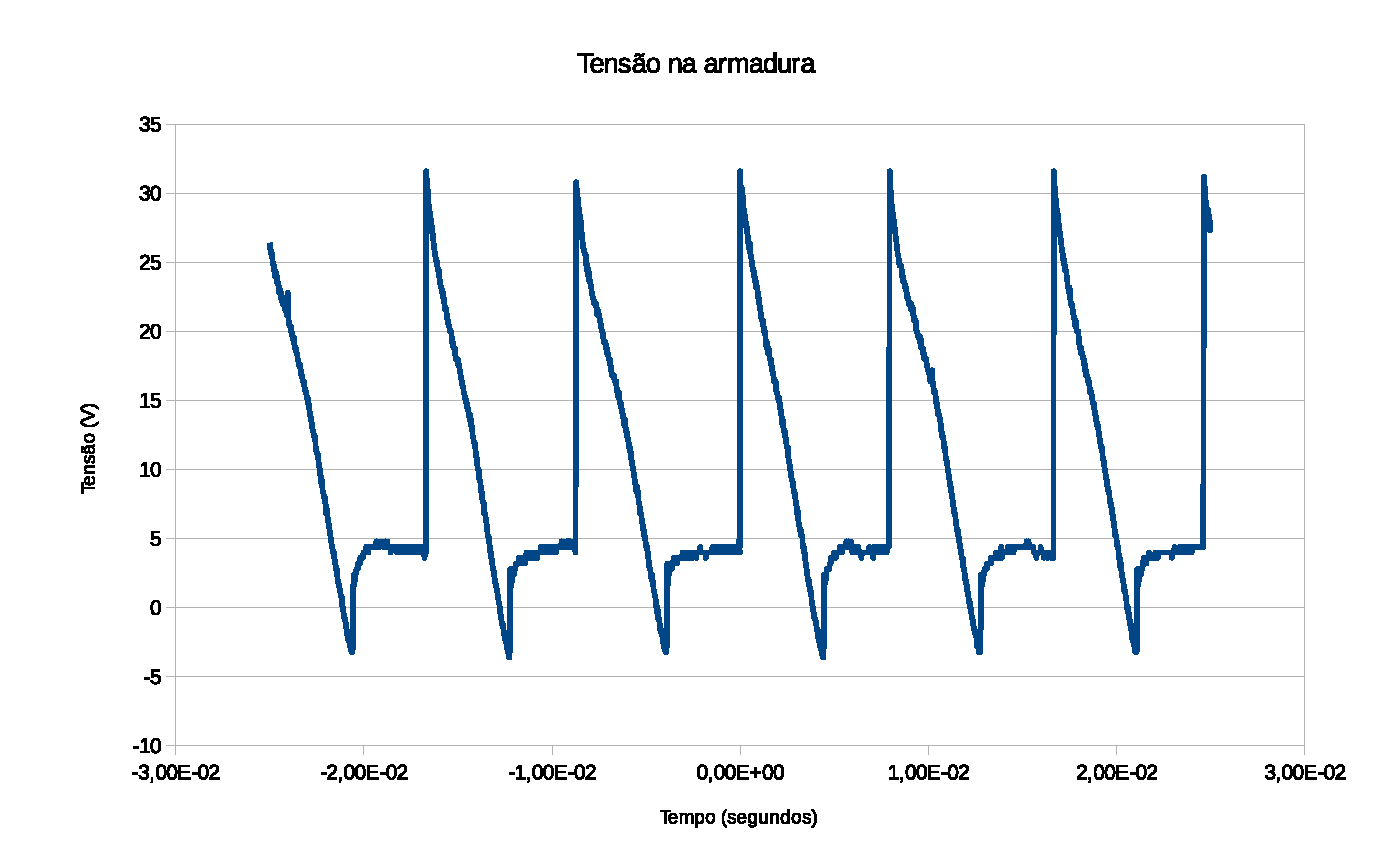
\includegraphics[width=\linewidth]{Dados/Retificador/1}
	\caption{Tensão de armadura do motor DC com retificador controlado para $\alpha=90^\circ$}
	\label{fig:varet}
\end{figure}

\begin{figure}[H]
	\centering
	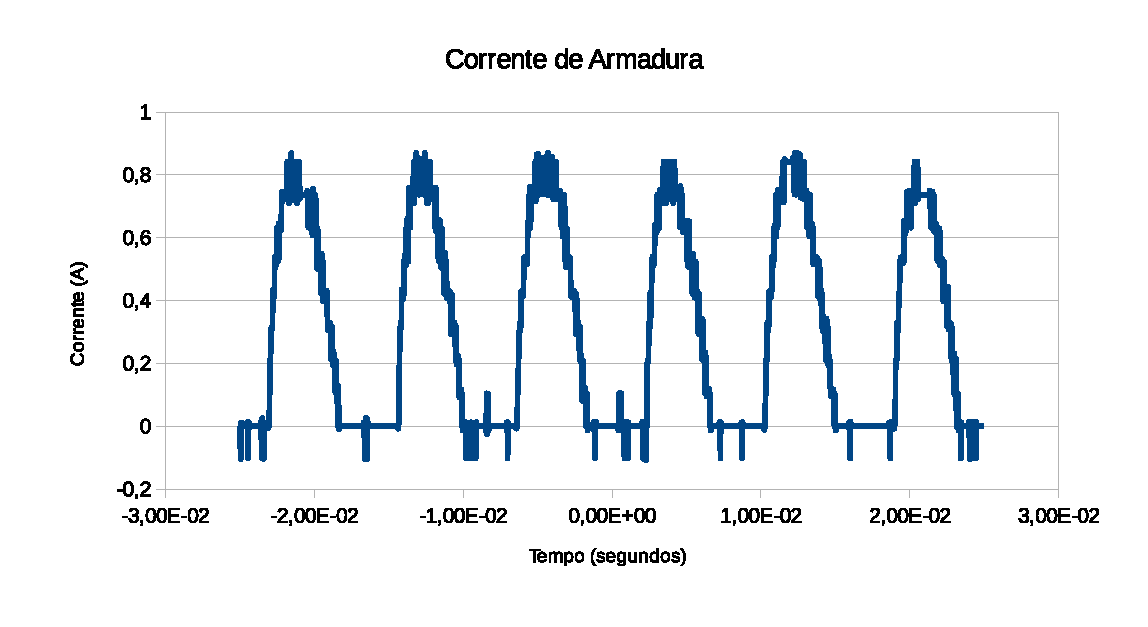
\includegraphics[width=\linewidth]{Dados/Retificador/corrente}
	\caption{Corrente no resistor de medição para $\alpha=90^\circ$}
	\label{fig:iaret}
\end{figure}

\begin{table}[H]
	\centering
	\caption{Tensão de armadura $v_a$, velocidade angular $\omega_m$, corrente de armadura $i_a$ e torque $T_m$ do motor DC para diferentes ângulos de disparo $\alpha$}
	\label{tab:varet}
	\begin{tabular}{|l|l|l|l|l|}
		\hline
		$\alpha$    & $v_a (V)$ & $\omega_m (rpm)$ & $i_a  (A)$ & $T_m (N\cdot m)$ \\ \hline
		$60^\circ$  & 4.81      & 340              & 0.248         & 0.0133           \\ \hline
		$70^\circ$  & 5.9       & 470              & 0.279         & 0.0149           \\ \hline
		$80^\circ$  & 7.12      & 650              & 0.297         & 0.0159           \\ \hline
		$90^\circ$  & 8.5       & 900              & 0.295     & 0.0158     \\ \hline
		$100^\circ$ & 9.8       & 1150             & 0.286         & 0.0153           \\ \hline
		$110^\circ$ & 10.6      & 1350             & 0.258         & 0.0138           \\ \hline
		$120^\circ$ & 11.6      & 1510             & 0.267         & 0.0143           \\ \hline
	\end{tabular}
\end{table}

Notamos que a variação da tensão na armadura é abrupta, e que chega a ficar abaixo dos $0\ V$, efeito introduzido pelo fator indutivo da carga, em alguns momentos. A corrente aplicada no motor chega a zerar em alguns momentos, o que não é desejado no acionamento do motor DC.

Variando o valor de $\alpha$, podemos observar que ocorre um aumento na tensão de armadura, e consequentemente, aumento na velocidade angular $\omega_m$. 

Se desconsiderarmos o atrito de coulomb, temos que:
\begin{equation}
	T_m = J\frac{d\omega_m}{dt} + B\omega_m + T_{wl}
\end{equation}
Sabemos que a carga acoplada também é da forma:
\begin{equation}
	T_{wl} = J_{wl}\frac{d\omega_m}{dt} + B_{wl}\omega_m
\end{equation}
Considerando que estamos trabalhando em regime permanente, podemos escrever:
\begin{equation}
T_m = (B + B_{wl})\omega_m
\end{equation}
Encontramos então que (para $\alpha = 70^\circ$)
\begin{equation}
	B + B_{wl} = 0.0003 N\cdot m\cdot s/rad
\end{equation}
Simulamos então um sistema com $R_a = R_a + R_R$, $B = B + B_{wl}$ e $k_t = k_e = 0,0536$ (considerando valores de indutância de armadura e inércia do motor bem baixos pois só nos interessamos no regime permanente) e encontramos a velocidade do motor em função do ângulo de disparo para simulação. Comparamos esse resultado com a curva que aproxima a velocidade do motor em função do ângulo de disparo calculada a partir dos dados apresentados na tabela \ref{tab:varet} e representada na equação \ref{eq:retdisp}. Os resultados são apresentados na figura \ref{fig:retalfa}.
\begin{equation}
	\omega_m [rad/s] = 289,5 - 2,158 \alpha [^\circ]
	\label{eq:retdisp}
\end{equation}

\begin{figure} [H]
	\centering
	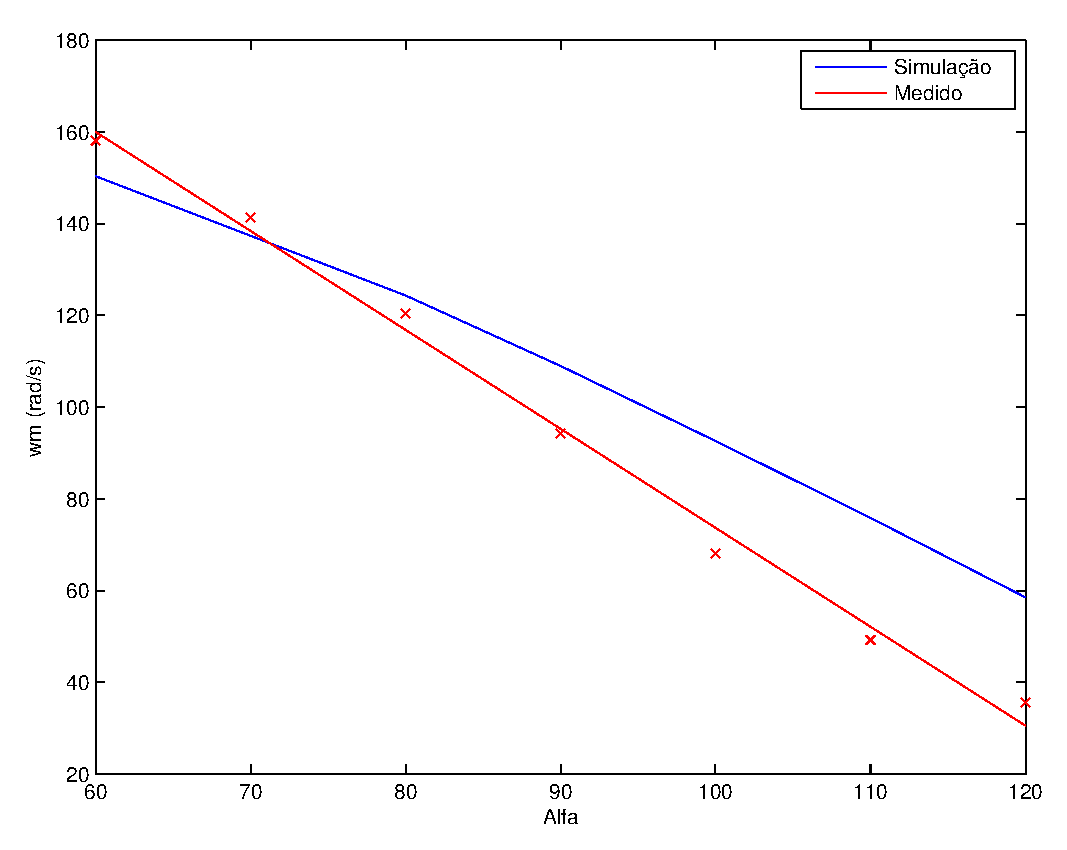
\includegraphics[width=\linewidth]{Dados/Retificador/walfa}
	\caption{Velocidade em função de $\alpha$ para retificador medido e simulado}
	\label{fig:retalfa}
\end{figure}

Como podemos ver, nosso modelo medido e simulado difere razoavelmente. Acreditamos que isso acontece pois adotamos uma série de simplificações no cálculo dos parâmetros do motor (por exemplo no calculo do coeficiente de atrito), além das imprecisões de medidas e diversos outros fatores. A curva linearizada da velocidade em função do ângulo de disparo ainda assim parece ser uma aproximação boa o suficiente dado que nos mantenhamos em um intervalo de valores para $\alpha$ apropriado.
\subsection{Conversor Step-Down}
Para o experimento com o conversor step-down, configuramos as tensões da fonte DC e pulsos do gerador de sinal. Ligamos o lado alto do conversor em $12\ V$, e o lado baixo na armadura do motor em série com o resistor de medição. Alimentamos o circuito de acionamento do conversor com $15\ V$ e ligamos o gerador de sinal nos cabos indicados por "BUCK" e "GND".

Utilizamos o mesmo motor do caso anterior, mas outra resistência de medição:

\begin{equation}
R_S=5.3\ \Omega
\end{equation}

Ligamos o circuito e capturamos a forma de onda da tensão de armadura $v_a$ para $D=50\%$, conforme figura \ref{fig:vabuck}. Variando os valores de $D$, obtivemos os valores da tabela \ref{tab:vabuck}. Prosseguimos o experimento registrando os valores de tensão na resistência de medição. A forma de onda para a corrente $i_a$ é mostrada na figura \ref{fig:iabuck}, para realizar o cálculo de $i_a$, utilizamos equação a seguir.

\begin{equation}
i_a=\frac{v_R}{R_S}
\end{equation}

Para cálculo do torque, utilizamos a equação \ref{eq:conserv}, levando em consideração apenas a conservação de energia e que os termos indutivos da carga seriam anulados uma vez que estamos trabalhando com valores médios e em regime permanente.

\begin{figure}[H]
	\centering
	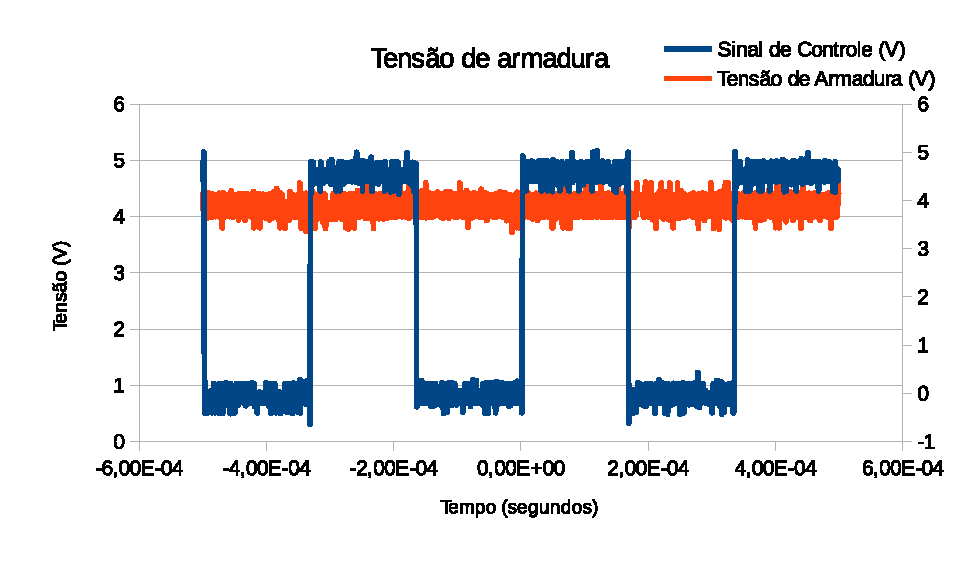
\includegraphics[width=\linewidth]{Dados/Buck/va}
	\caption{Tensão de armadura do motor DC com chopper em step-down para $D=50\%$}
	\label{fig:vabuck}
\end{figure}

\begin{figure}[H]
	\centering
	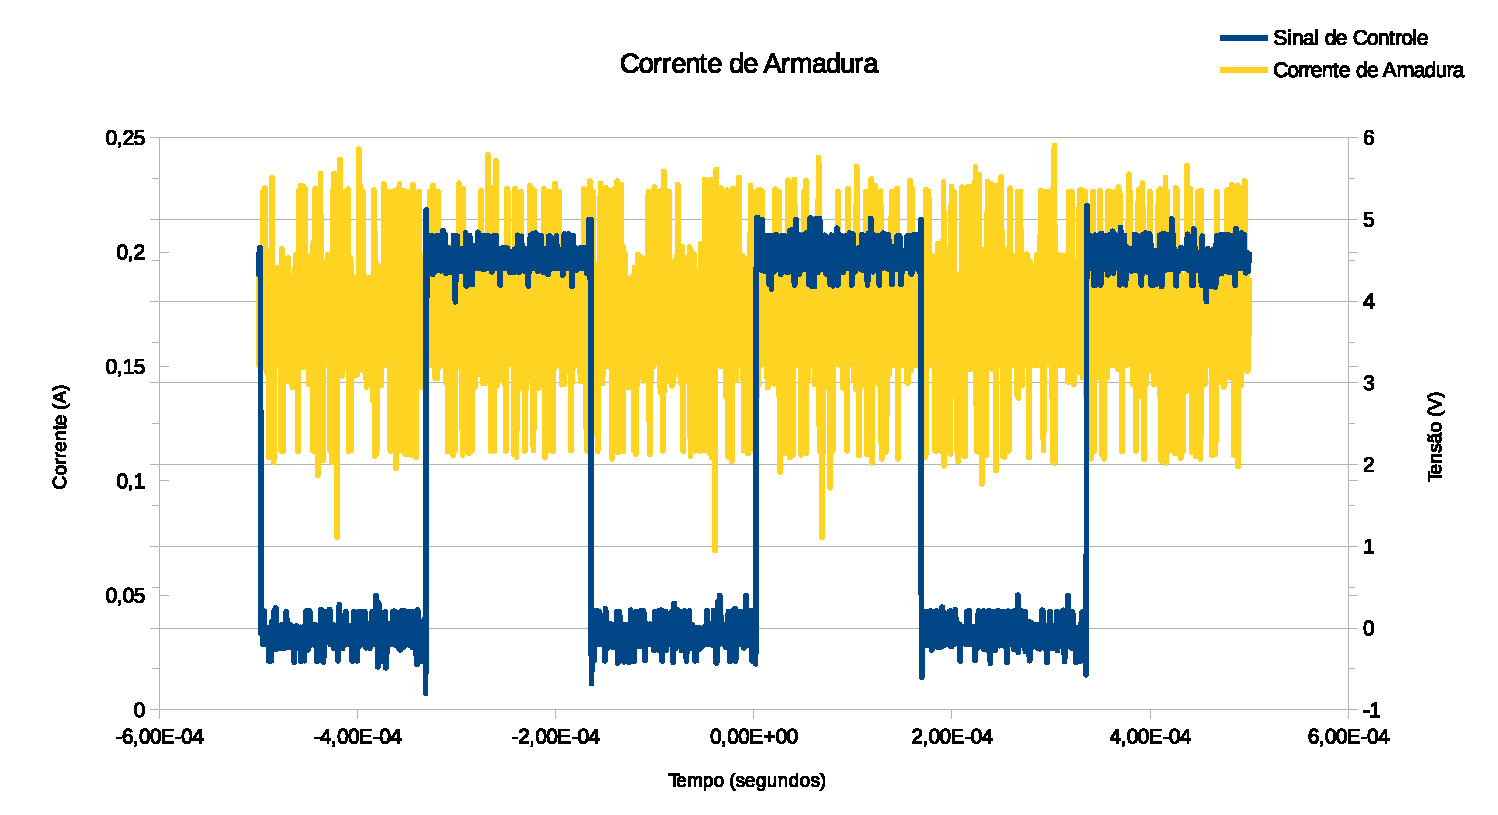
\includegraphics[width=\linewidth]{Dados/Buck/ia}
	\caption{Corrente no resistor de medição para $D=50\%$}
	\label{fig:iabuck}
\end{figure}

\begin{table}[H]
	\centering
	\caption{Tensão de armadura $v_a$, velocidade angular $\omega_m$, corrente de armadura $i_a$ e torque $T_m$ do motor DC para diferentes duty-cycles $D$}
	\label{tab:vabuck}
	\begin{tabular}{|l|l|l|l|l|}
		\hline
		$D$    & $v_a (V)$ & $\omega_m (rpm)$ & $i_a (A)$ & $T_m (N\cdot m)$ \\ \hline
		$20\%$ & -     & -          & -         & -           \\ \hline
		$30\%$ & 2.18  & 102        & 0.117     & 0.0137      \\ \hline
		$40\%$ & 3.08  & 234        & 0.143     & 0.0114       \\ \hline
		$50\%$ & 4.32  & 390        & 0.170     & 0.0124       \\ \hline
		$60\%$ & 5.4   & 574        & 0.192     & 0.0124       \\ \hline
	\end{tabular}
\end{table}

Como podemos ver a tensão e a corrente aplicada sobre o motor se mantém praticamente constantes, fator altamente desejável no controle desses dispositivos pois assim nossa velocidade e torque apresentarão menos variações.

Usando o mesmo raciocínio que utilizamos para o retificador, calculamos os valores de $k_t$ e $B + B_{wl}$. Notamos uma variação significativa em ambos os parâmetros, provando que nossas hipóteses simplificadoras só podem ser aplicadas quando não nos afastamos muito da nossa condição de operação em que elas foram feitas (no caso do retificador e do buck estamos operando em duas regiões bastante distintas), e simulamos o sistema para um motor com os parâmetros encontrados $R_a = R_a + R_s$, $B = B + B_{wl} = 0,00046$ e $k_t = k_e = 0,07$.  Comparamos esse resultado com a curva que aproxima a velocidade do motor em função do ângulo de disparo calculada a partir dos dados apresentados na tabela \ref{tab:vabuck} e representada na equação \ref{eq:buckdisp}. Os resultados são apresentados na figura \ref{fig:buckwd}.
\begin{equation}
\omega_m [rad/s] = 40,05 + 1,65 D [\%]
\label{eq:buckdisp}
\end{equation}

\begin{figure} [H]
	\centering
	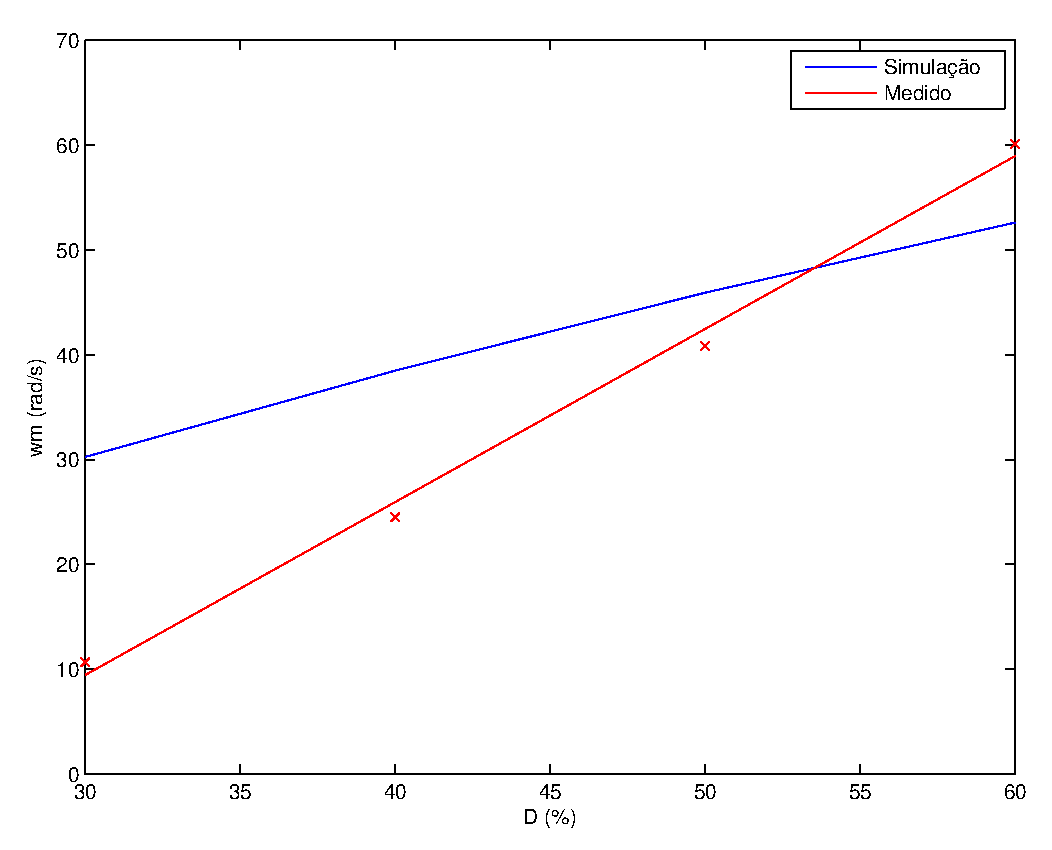
\includegraphics[width=\linewidth]{Dados/Buck/wd}
	\caption{Velocidade em função do duty-cycle para conversor buck medido e simulado}
	\label{fig:buckwd}
\end{figure}

Como podemos ver, nosso modelo medido e simulado difere razoavelmente. Acreditamos que isso acontece pois adotamos uma série de simplificações no cálculo dos parâmetros do motor (por exemplo no calculo do coeficiente de atrito), além das imprecisões de medidas e diversos outros fatores. A curva linearizada da velocidade em função do ângulo de disparo ainda assim parece ser uma aproximação boa o suficiente dado que nos mantenhamos em um intervalo de valores para $D$ apropriado.

% e
A carga acoplada ao motor DC (motor AC interligado pelo eixo) funciona para criar torque e aumentar a corrente de armadura. Também faz com que a velocidade de rotação seja diminuída.
% f
O conversor monofásico controlado de onda completa opera em dois quadrantes uma vez que ele não permite a inversão da corrente aplicada no motor. O chopper operando em step-down, por sua vez, opera só no primeiro quadrante, com tensão e corrente positivas.
\end{document}

